\documentclass[12pt, a4paper, twoside]{report}
\usepackage[left=3cm, right=2.5cm, top=2.5cm, bottom=2.5cm]{geometry}
\usepackage{amsmath}
\renewcommand{\baselinestretch}{1.3} 
\usepackage{amssymb}
\usepackage{amsthm}
\usepackage[]{longtable}
\usepackage{enumerate}
\usepackage{array}
\usepackage[pdftex]{graphicx}
\usepackage{indentfirst}
\usepackage{booktabs}
\usepackage{color}
\usepackage{parskip}
\usepackage{pgfplots}
\usepackage{titlesec}
\usepackage[]{gensymb}
\usepackage{fancyhdr}
% \usepackage{vcell}
\usepackage{microtype}
\usepackage[pdftex]{hyperref}
\usepackage[T1]{fontenc}
% \usepackage[T1]{polski}
\usepackage[utf8]{inputenc}
\usepackage[]{lmodern}
\usepackage[]{textcomp}
\usepackage{subcaption}
\usepackage{multirow}
\usepackage[]{afterpage}
\usepackage{listings}
\captionsetup{compatibility=false}
\lstset{ %
  language=Python,
  basicstyle=\footnotesize\ttfamily,
  numbers=left,
  stepnumber=1,
  showstringspaces=false,
  tabsize=1,
  columns=fullflexible,
  frame=single,
  breaklines=true,
  postbreak=\mbox{\textcolor{red}{$\hookrightarrow$}\space},
}
\usepackage{fancyhdr}
\pagestyle{fancy}
\fancyhead[RO, LE]{\thepage}
\fancyhead[RE, LO]{}
\fancyfoot{}
\renewcommand\headrulewidth{0pt}
\renewcommand\footrulewidth{0pt}

\newcommand{\bibTitle}[1]{``#1''}
    
\def\blankpage{%
      \clearpage%
      \thispagestyle{empty}%
      %\addtocounter{page}{0}%
      \null%
      \clearpage}

\fancypagestyle{plain}{%
\fancyhf{}% clears all header and footer fields
\fancyhead[LE,RO]{\thepage}%
\renewcommand{\headrulewidth}{0pt}%
\renewcommand{\footrulewidth}{0.4pt}}


\titleformat{\chapter}[display]
  {\normalfont\Large\raggedleft}
  {\MakeUppercase{\chaptertitlename}
    \rlap{ \resizebox{!}{1.5cm}{\thechapter} \rule{5cm}{1.5cm}}}
  {10pt}{\Huge}
\titlespacing*{\chapter}{0pt}{30pt}{50pt} % odstępy w tytule głównym

\begin{document}

\begin{titlepage}
\begin{center} % wypośrodkuj
\Large \textbf{WOJSKOWA AKADEMIA TECHNICZNA}\\[1mm]
\Large {WYDZIAŁ CYBERNETYKI}\\[1mm]
\end{center}

\vspace{0.5cm}
\begin{center}
	
\includegraphics[scale= 0.3]{Obrazy/Logo_WAT.jpg} % wstawia wycentrowany plik graficzny 	<logo.pdf> z podkatalogu <graphics> i ustawia jest wysokość (zachowując proporcje) równą 3 cm
\end{center}
\begin{center}
	\Huge {Praca dyplomowa magisterska} \\
	\vspace{0.5cm}
	Mobilny system zarządzania i sterowania bezpilotowym statkiem latającym
\end{center}

\vspace{0.5cm} % wstawia odstęp pionowy 

\begin{center}
	\Large {Norbert Waszkowiak}
\end{center}


\vspace{1cm}
%\hfill

\hfill
\begin{minipage}[t]{0.45\textwidth}
	\begin{flushleft}
		\begin{Large}
			\textbf  {Promotor}: \\ 
			dr inż. Michał Dyk \\
			\vspace{0.5cm}
			Potwierdzam przyjęcie pracy
		\end{Large}
	\end{flushleft}
\end{minipage}

\vspace{4cm}

\begin{center} 
Warszawa, 2022
\end{center}

\end{titlepage}

  % Spis treści ]\\\\\\\\\\\\\\\\

\tableofcontents % wstawia spis treści


 % Główna część pracy \\\\\\\\\\\\
 
\chapter*{Wstęp} % rozdział nienumerowany (dlatego *)
\addcontentsline{toc}{chapter}{Wstęp} % uwzględnia nienumerowany rozdział <Wstęp> w <Spisie treści>
\hspace{1cm}Wstep - text

Zadania do zrealizowania w pracy:
\begin{itemize}
\item Prezentacja zagadnienia BSP oraz koncepcji ich wykorzystania;
\item Przegląd i prezentacja technologii mobilnych z uwzględnieniem aspektów tworzenia aplikacji i komunikacji M2M;
\item Projekt mobilnego systemu zarządzania i sterowania bezpilotowym statkiem latającym;
\item Implementacja systemu;
\item Testy systemu oraz prezentacja użycia na wybranym case study.
\end{itemize}
\newpage	

\chapter{Prezentacja zagadnienia bezpilotowych statków latających oraz koncepcji ich wykorzystania}
\hspace{1cm}text
\section{Historia BSP}
\hspace{1cm}text
\section{Technologia i producenci BSP}
\hspace{1cm}text
\section{Zastosowania BSP}
\hspace{1cm}text
\section{Dostosowywanie drona do wymagań użytkownika}
\hspace{1cm}text

% \section{}
% \subsection{}

\chapter{Przegląd i prezentacja technologii mobilnych z uwzględnieniem aspektów tworzenia aplikacji i komunikacji M2M}
\hspace{1cm}W tym rozdziale przedstawiono technologie komunikacji bezprzewodowej wykorzystywane w komunikacji M2M, ze szczególnym uwzględnieniem komunikacji pomiędzy bezzałogowym statkiem powietrznym, a kontrolerem. Analizę wykorzystywanych rodzajów komunikacji dokonano na podstawie oferty najpopularniejszego producenta dronów konsumenckich DJI.

\section{Komunikacja M2M}
\hspace{1cm}Komunikacja M2M (machine-to-machine) służy do definiowania technologi, która umożliwia wymianę informacje pomiędzy urządzeniami w sieci bez jakikolwiek ingerencji ludzi. Sztuczna inteligencja wraz z metodami uczenia maszynowego znacznie ułatwia takie procesy, między innymi umożliwia ona podejmowanie autonomicznych decyzji przez te urządzenia. Ta komunikacja jest podstawą istnienia IoT.\cite{m2m-web}

\subsection{Cel}
\hspace{1cm}Głównym celem M2M jest przenoszenia danych z sensorów do sieci. W porównaniu do innych technolgi, które umożliwiają monitorowanie zasobów, korzysta ona często z dostępnych publicznie sieci np. GSM, co redukuje jej koszty utrzymania. Można wyróżnić 3 elemnty takiego systemu:
\begin{itemize}
  \item łącze do przesyłu danych, np. WiFi, GSM, RFID
  \item sensory, np. czujnik temperatury, kamera
  \item oprogramowaie, które umożliwia podejmowanie zautmatyzowanych decyzji
\end{itemize}
\hspace{1cm}Najpopularniejszą dziedziną tej technologii, jest telemetria. Jej celem jest pomiar wybranej wielkości i jej przesyłanie do centralnej jednostki, oddalonej od miejsca pomairu. Na początku do tego celu były wykorzystywane linie telefoniczne, a następnie radiowe. Rozwój technologi, a w tym łączności bezprzewodowej sprawił, że rola wykorzystywania telemetrii w nauce inżynierii i produkcji poszerzyła się do użytku codziennego w jednostkach grzewczych, mierników elektrycznych i wszelkich urządzeń podłączonych do internetu.\cite{m2m-web}

\subsection{Wymagania}
\hspace{1cm}Według Europejskiego Instytutu Norm Telekomunikacyjnych (ETSI) komunikacja M2M musi spełniać następujące wymagania:
\begin{itemize}
  \item \textbf{Skalowalność}: w miarę dołączania kolejnych urządzeń do systemu system nadal musi funkcjonować;
  \item \textbf{Anonimowość}: na każde żądanie, w związku z wymaganiami prawnymi system musi umożliwiać ukrywanie tożsamości urządzenia;
  \item \textbf{Logowanie}: ważne wydarzenia w systemie, takie jak: pojawienie się błędnych informacji czy nieudane próby instalacji, muszą być zarejestrowane, a rejestry te muszą być dostępne na żądanie;
  \item \textbf{Zasady komunikacji między aplikacjami}: aplikacje w systemie powinny mieć możliwość komunikowania się. W szczególności bramki i urządzenia końcowe komunikujące się za pomocą technologi SMS czy Ethernet powinny komunikować
  się za pomocą połączenia P2P (peer-to-peer);
  \item  \textbf{Metody dostarczania}: w ramach systemu powinny być dostarczane metody komunikacji takie jak: \emph{unicast}, \emph{multicas}, \emph{broadcast} i \emph{annycast}, a wszędzie gdzie to możliwe metoda \emph{broadcast} powinna być zastąpiona za pomocą \emph{multicast}, tak aby zminimalizować obciążenie sieci;
  \item \textbf{Harmonogram przesyłania komunikatów}:  dostęp do sieci powinien być kontrolowany, tak samo, jak harmonogram przesyłania komunikatów. Sam system powinien również uwzględniać obciążenia aplikacji M2M w harmonogramie przesyłania wiadomości;
  \item \textbf{Wybór ściezek komunikacjynych}: ścieżki w systemie powinny zapewniać optymalizacje bazującą na: awariach transmisji, kosztu i opóźnieniach, w momencie, gdy istnieją inne ścieżki do punktu docelowego. \cite{m2m-web}
\end{itemize}

\section{Technologie komunikacji M2M}
\hspace{1cm}Gdyby w technologi tak samo, jak w literaturze występowały epoki, aktualnie znajdowalibyśmy się w epoce połączonych ze sobą obiektów. IoT (Internet of Things) zdobywa aktualnie coraz więcej uwagi nie mal w każdej domenie, a szczególnie w takich jak biznes, elektronika konsumencka, przemysł czy transport. Niemal każdy obiekt elektryczny w dzisiejszym świecie jest ze sobą połączony w ten czy inny sposób. Siedząc w biurze, za pomocą dostarczanych aplikacji, możemy kontrolować drzwi, bramę garażową, czajnik elektryczny czy rolety okienne w naszym domu. W mieście kontrolujemy kamery i oświetlenie z odległych lokacji. IoT odgrywa w tym ważną rolę, ponieważ to ono umożliwia łączenie przeróżnych obiektów, za pomocą sieci połączeń i wymianę danych między nimi.\cite{LoRa-article}

\subsection{Ogólna klasyfikacja technolgi M2M}
\hspace{1cm}Poniżej przedstawiono ogólne porównanie technologi komunikacyjnych M2M.

\begin{table}[!htbp]
  \resizebox{\textwidth}{!}{%
  \begin{tabular}{|l|l|l|l|}
  \hline
  \textbf{}            & \begin{tabular}[c]{@{}l@{}}\textbf{Local Area Network}\\ Komunikacja krótko \\ dystansowa\end{tabular}            & \begin{tabular}[c]{@{}l@{}}\textbf{Low Power Wide Area}\\ Intenet Of Things\end{tabular}            & \begin{tabular}[c]{@{}l@{}}\textbf{Celluar Network}\\ Tradycyjne M2M\end{tabular}                               \\ \hline
  \textbf{Użycie}      & 40\%                                                                                                              & 45\%                                                                                                & 15\%                                                                                                            \\ \hline
  \textbf{Zalety}      & \begin{tabular}[c]{@{}l@{}}- Dobrze ugruntowana norma\\ - W budynkach\end{tabular}                                & \begin{tabular}[c]{@{}l@{}}- Niskie zużycie energi\\ - Niskie koszty\\ - Pozycjonowanie\end{tabular} & \begin{tabular}[c]{@{}l@{}}- Istniejące pokrycie znacznego \\ obszaru\\ - Duża prędkość transmisji\end{tabular} \\ \hline
  \textbf{Wady}        & \begin{tabular}[c]{@{}l@{}}- Wysokie zużycie energi \\ elektrycznej\\ - Duży koszt sieci i zależności\end{tabular} & \begin{tabular}[c]{@{}l@{}}- Niska prędkość transmisji\\ - Wschodzący standard\end{tabular}         & \begin{tabular}[c]{@{}l@{}}- Wysoki koszt posiadania\\ - Mała autonomia\end{tabular}                            \\ \hline
  \textbf{Technologia} & Bluetooth, WiFi                                                                                                   & LoRa                                                                                                & GSM, 3G, 4G, 5G                                                                                                 \\ \hline
  \end{tabular}%
  }
  \caption{Porównanie rodzajów technolgi M2M.\cite{LoRa-article}}
\end{table}

\subsection{LoRa}
\hspace{1cm}LoRa (Long Range) to nowa technologia połączeń bezprzewodowych w świecie IoT, która ostatnio ewoluowała i zyskała szczególną popularność, w urządzeniach z ograniczoną pojemnością elektryczną umożliwiając systemom wbudowanym przesyłanie małej ilości danych na dużych dystansach w krótkich interwałach czasowych.

\hspace{1cm}Komunikacja w aplikacjach IoT jest dzisiaj wykonywana w przeróżnych technologiach, a każda z nich ma swoje zalety, funkcje, a przez to też przeznaczenie. Żadna z tych technolgi nie może pokryć całego zapotrzebowania świata IoT, ponieważ wszystkie one posiadają cechy, które czynią je odpowiednie dla postawionego konkretnego zadania.

\hspace{1cm}WiFi to najpopularniejsza technologia komunikacji bezprzewodowej, która ewoluowała przez wiele lat i jest wykorzystywana przede wszystkim do komunikacji na dużych
odległościach. Na krótkie dystanse mamy przeznaczone do tego no. Bluetooth czy ZigBee. We wszystkich z nich największą wadą jest duże zużycie energii elektrycznej. Technologia Lora zapewnia bezpieczne, mobilne dwukierunkowe połączenie o niskim koszcie elektrycznym, wykorzystywane jest ono w IoT, szczególnie w domenie smart city, czy nawet ogólnej komunikacji M2M. LoRa zalicza się do LPWA(Low Power Wide Area), czyli rodzaju bezprzewodowej rozległej sieci telekomunikacyjnej, stworzonej w celu umożliwienia komunikacji na duże odległości przy niskiej przepływności i niskim poborze energii. \cite{LPWA-wiki} W tego typu komunikacji wyróżnia się LoRa ze względu na jej:
\begin{itemize}
  \item długodystansowość;
  \item dwukierunkowość;
  \item wysoką pojemność węzłów w sieci;
  \item długość życia na baterii;
  \item odporność interfejsów;
  \item bezpieczeństwo i efektywność sieci. \cite{LoRa-article}
\end{itemize}


\subsubsection{Cechy}
\hspace{1cm}Technologie tą wyróżniają następujące cechy:
\begin{itemize}
  \item Pojedyncza bramka może pokryć obszar aż $100km^2$;
  \item Oferuje ona podwójne szyfrowanie AES;
  \item Bazuje na technologi CSS (widmo rozproszone Chrip), które umożliwia śledzenie obiektów i jest odporne na zanikanie sygnałów;
  \item Topologia gwiazdy eliminuje zanikanie danych przez urządzenia pośrednie, co przyczynia się do zmniejszenia poboru mocy. \cite{LoRa-article}
\end{itemize}


\subsubsection{Ograniczenie przepustowości}
\hspace{1cm}W sieci LoRa wszystkie klasy ramek wymagają potwierdzenia, co wiąże się z tym, że po każdym potwierdzeniu ramko przez urządzenie końcowe w dowolnym oknie czasowym następuje okres wyłączenie, w celu zachowanie zgodności z przepisami dotyczącymi cyklu pracy. W związku z tym, aby uniknąć wyczerpania limitu pojemności przez sieć i urządzenia końcowe, muszą one ograniczyć liczbę potwierdzeń. Również w podsieciach LoRa po przesłaniu danych następuje okres wyłączenia, w którym na danym kanale nie są wysyłane żadne dane. Te dwa okresy, tzn. okres wysyłania danych i wstrzymania transmisji stanowi cykl pracy, dlatego  to w sieci LoRa przepustowość jest ograniczona cyklem pracy.\cite{LoRa-article}

\subsection{Narow band IoT}
\hspace{1cm}Wraz z rozwojem świata IoT NB-IoT stało sie wiodącą technologią komunikacji komórkowej dla zdalnych pomiarów w całej Europie. NB-IoT to technologia dostępu radiowego, która ponownie używa komponentów stworzonych przez jej poprzednika LTE, aby umożliwić jej działa na licencjonowanej częstotliwości. Może ona również działać w trybie autonomicznym. Tak jak sama nazwa wskazuje, cały system działa w wąskim spektrum częstotliwości, bo tylko w 200kHz, co wprowadza elastyczność zastosowań dzięki minimalnym wymaganiom częstotliwości, w porównaniu do jej poprzednika LTE. Cała szerokość 200kHz została podzielona na kanały po 3.75 kHz lub 15 kHz, co umożliwia połączenie w bardzo wysoką prędkość nadawania, a także daleki zasięg połącznika, biorąc pod uwagę wąskie widmo sygnału. \cite{nbiot-article}  

\subsection{NB-IoT vs Lora}

\begin{table}[!htbp]
  \resizebox{\textwidth}{!}{%
  \begin{tabular}{|l|c|c|}
  \hline
  \textbf{Parametr}                                                                     & \textbf{LoRa}               & \textbf{NB-IoT}       \\ \hline
  \textbf{Pasmo}                                                                        & 125 kHz                     & 180 kHz               \\ \hline
  \textbf{Pokrycie}                                                                     & 165 dB                      & 164 dB                \\ \hline
  \textbf{Żywotność baterii}                                                            & 15+ lat                     & 10+ lat               \\ \hline
  \textbf{\begin{tabular}[c]{@{}l@{}}Maksymalne natężenie \\ elektryczne\end{tabular}}  & 32 mA                       & 120 mA                \\ \hline
  \textbf{\begin{tabular}[c]{@{}l@{}}Spoczynkowe natężenie \\ elektryczne\end{tabular}} & 1 µA                        & 5 µA                  \\ \hline
  \textbf{Przepustowość}                                                                & 50 Kbps                     & 60 Kbps               \\ \hline
  \textbf{Opóźnienie}                                                                   & Zależne od klasy urządzenia & 10 s                  \\ \hline
  \textbf{Bezpieczeństwo}                                                               & AES 128 bit                 & 3GPP (128 to 256 bit) \\ \hline
  \textbf{Geolokalizacja}                                                               & Tak (TDOA)                  & Tak (In 3GPP Rel 14)  \\ \hline
  \textbf{Jakość/cena}                                                                  & Wysoka                      & Średnia                \\ \hline
  \end{tabular}%
  }
  \caption{Porównanie technologi LoRa i NB-IoT \cite{NB-IoT_vs_Lora}}
  \end{table}

\hspace{1cm}Zarówno LoRa jak i NB-IoT należą do wspomnianej wcześniej technologi LPWAN. Podstawowa różnice pomiędzy tymi dwoma technologiami można dostrzec w zużyciu baterii, prędkości transmisji i opóźnień.

\section{Komunikacja bezprzewodowa w dronach konsumenckich}
\hspace{1cm}Shenzhen DJI Sciences and Technologies Ltd., znany powszechnie pod nazwą handlową DJI, jest obecnie największym rpoducentem dronów konsumenckich. W 2020r. firma ta posiadała 70\% udziału w światowym rynku. \cite{dji-wiki} Przeglądając katalog ich produktów, można wyróżnić tylko 3 technologie komunikacji bezprzewodowej: wzomocnione WiFi (ang. enhanced WiFi), Lightbridge, OcuSync.

\subsection{WiFi}
\hspace{1cm}WiFi nie zostało wprowadzone ściśle do komunikacji bezprzewodowej statków powietrznych, ale odnajduje się w tym całkiem dobrze. Jest ona wykorzystywana głównie w bardziej budżetowych wersjach dronów, ze względu na możliwość skorzystanie przez producenta z posiadanej przez użytkownika infrastruktury (smartfonów), czy niskiej ceny komponentów.

\hspace{1cm}Przykładowo dron \emph{DJI Tello}, który jest najtańszą opcją dostępną od producenta DJI, przeznaczoną głównie do nauki latania, a nawet praktycznie programowania przez najmłodszych pasjonatów, nie posiada on w zestawie dedykowanego kontrolera. Kontrolowanie drona odbywa się za pomocą aplikacji na smartfona, która łączy się z dronem za pomocą WiFi tak jak do punktu dostępowego z internetem. Zasięg takiego połączenia według producenta to 100m \cite{dji-store}.


\begin{figure}[!htbp]
  \centering
  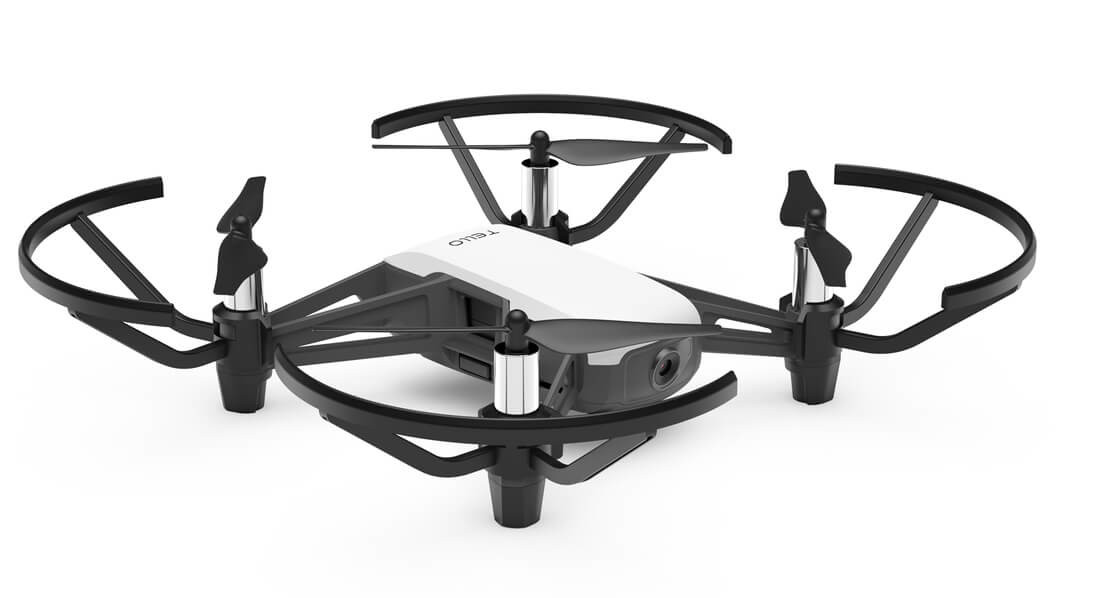
\includegraphics[width=10cm]{Obrazy/dji-tello.jpg}
  \caption{DJI Tello\cite{dji-store}}
  \end{figure}

  \hspace{1cm}W swojej ofercie DJI ma również dostępnego drona \emph{DJI Mini SE}, który również korzysta z technologii WiFi, ale w swoim wyposażaniu posiada dedykowany do niego kontroler. Taka konfiguracja pozwala na uzyskanie zasięgu do 2 km. \cite{dji-mavic-mini-se-spec}

\hspace{1cm}WiFi jest także bardzo podatne na wszelkie zakłócenia, wynikające z ukształtowania terenu czy zaszumienia sieci pochodzącego z istniejących sieci domowych. Wyprodukowanie drona w tej technolgi jest najtańszą dostępną opcją, która umożliwia transmisje obrazu, jednak należy pamiętać, aby nie stawiać jej przy tym za dużych wymagań. WiFi stanowi bardzo dobry punkt startowy w komunikacji bezprzewodowej bezzałogowych statków powietrznych.

\subsection{Lightbridge}
\hspace{1cm}Lightbridge to technologia od DJI, która doczekała się jej dwóch wydań. Pierwszych wzmianek o niej można doszukiwać się w 2014 roku. \cite{lightbridge-dji}, a drugiego wydania już w 2015 roku\cite{lightbridge2-dji}. Obecnie nie jest już rozwijana, a producent skupił się na rozwoju jego drugiej technologi: OcuSync.

\hspace{1cm}Technologie prezentowane przez DJI mają parę cech zbliżające je do WiFi, przede wszystkim transmisja ta odbywa, gdyż odbywa się ona na tej samej częstotliwości: 2,4GHz. Była ona kierowana głównie do dronów z wyższego pułapu cenowego, dlatego że jej produkcja była bardzo kosztowna, a koszt wynikał z tego, że producent opracował to rozwiązanie na swoim autorskim układzie scalonym i oprogramowaniu. Wskutek czego pozwoliło to osiągnąć duże lepsze wyniki niż transmisja po WiFi. Zasięg lotu według producenta to odległość do 5km.

\subsection{OcuSync} 
\hspace{1cm}OcuSync został po raz pierwszy zademonstrowany przez producenta wraz z wydaniem drona \emph{Mavic Mini Pro}. Pierwsze wydanie tej technologi pozwalało na transmisje do 7km na częstotliwości 2,4GHz. Obraz mógł być przesyłany w rozdzielczości 720p i 1080p. Jakość fullHD była dostępna tylko na krótszych odległościach, gdy dystans się zwiększał, a dostępna prędkość transmisji spadała, dron przechodził automatycznie na transmisje w 720p. Opóźnienie było rzędu 160-170ms. A największą cechą wyróżniającą tę technologię była możliwość podłączenia jednocześnie dwóch kontrolerów i do 4 urządzeń odbiorczych.

\hspace{1cm}Kolejnym krokiem było wydane kolejnej wersji oznaczonej jako OcuSync 1.5, w której dodano transmisję również na częstotliwości 5Ghz. Zmniejszono także opóźnienia w transmisji. Dodatkowo technologia umożliwiał automatyczną zmianę kanałów komunikacyjnych w trakcie lotu na te najmniej obciążone. W pierwszej wersji kanał 
transmisji można było wybrać tylko przed startem bezzałogowego statku powietrznego.


\begin{figure}[!ht]
  \centering
  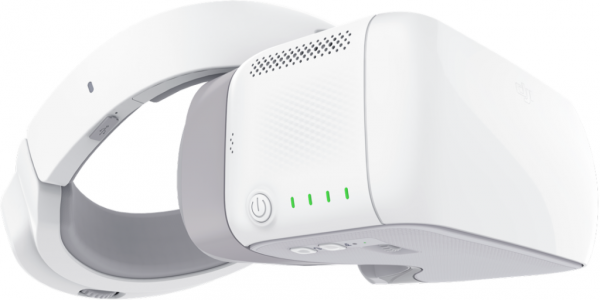
\includegraphics[width=8cm]{Obrazy/dji-google.png}
  \caption{Pierwsza wersja gogli do FPV od DJI \cite{dji-gogle}}
  \end{figure}
  

\begin{figure}[!ht]
  \centering
  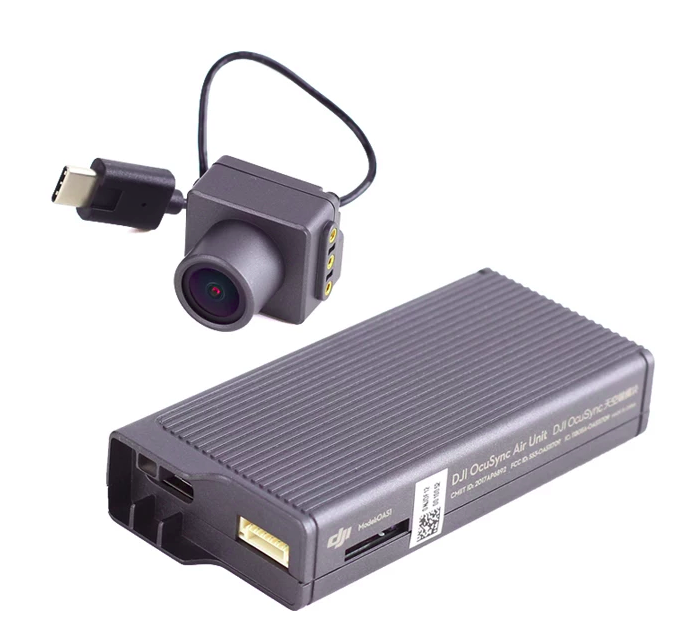
\includegraphics[width=8cm]{Obrazy/dji-air-unit.png}
  \caption{Dji OcuSync Air Unit\cite{dji-store}}
  \end{figure}
  

\hspace{1cm}Wraz z wydaniem nowej wersji zaprezentowano gogle DJI przeznaczone do transmisji obrazu w trybie FPV (ang. first person view, widok pierwszo-osobowy) i również OcuSync Aircraft System, czyli zintegrowanego systemu umożliwiającego sterowanie i transmisji obrazu z wykorzystaniem tej technologi w dronach i pojazdach DIY.

\hspace{1cm}Producent w trakcie swojej historii doprowadził do pewnych nieścisłości, mimo że dron \emph{Phantom 4 pro v 2.0} korzystał teoretycznie z najnowszej wersji OcuSync, ale nie posiadał on możliwości zmiany kanałów transmisji w trakcie lotu, opóźnienie zależało też od tego, czy korzystano z kontrolera dołączonego do zestawu, czy jego droższej, lepiej wyposażonej wersji: \emph{DJI RC Plus}.
  

\begin{figure}[!htbp]
  \centering
  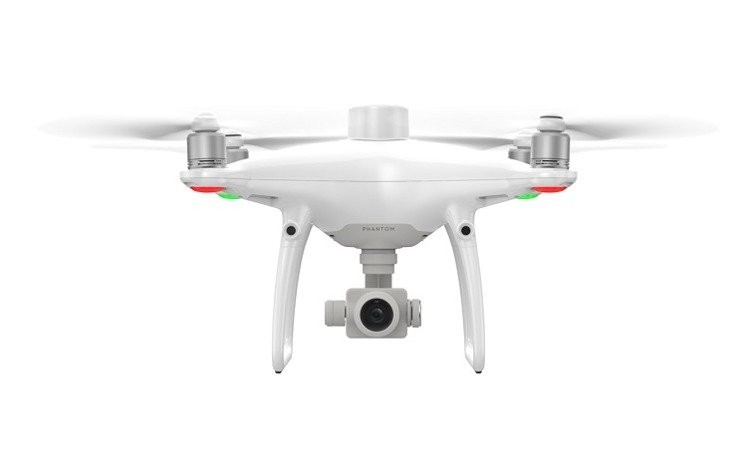
\includegraphics[width=8cm]{Obrazy/dji-phantom-v2.jpg}
  \caption{DJI Phantom v2.0\cite{dji-store}}
  \end{figure}
  

\begin{figure}[!htbp]
  \centering
  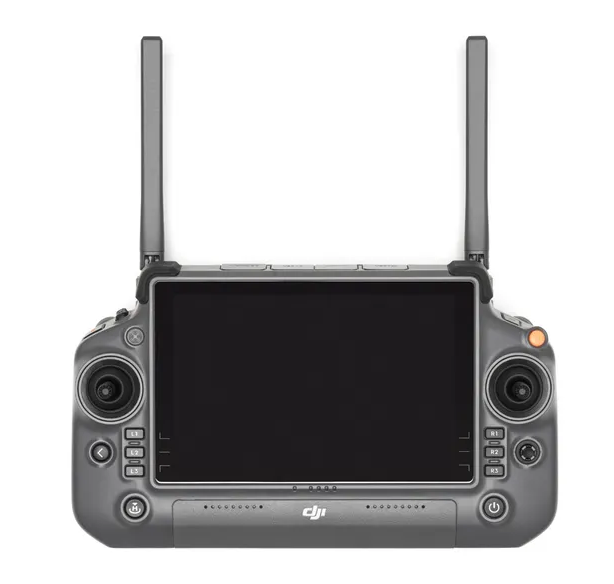
\includegraphics[width=8cm]{Obrazy/dji-rc-plus.png}
  \caption{DJI RC plus\cite{dji-store}}
  \end{figure}
  


\hspace{1cm}Wersja 2.0 wprowadziła dalsze ulepszenia, m.in. kontorlowanie dronów na jeszcze większe dystanse i z jeszcze mniejszymi opóźnieniami, a także kompatybilność wsteczną po aktualizacji oprogramowania.

\subsection{FHSS i  OFDM}

\hspace{1cm}Zarówno Lightbridge, jak i OcuSync używają szyfrowanej modulacji OFDM (ang. Orthogonal Frequency-Division Multiplexing, zwielokrotnianie z ortogonalnym podziałem częstotliwości)) dla transmisji obrazu i z formy FHSS (ang. Frequency-Hopping Spread Spectrum) dla transmisji sygnałów sterowania. Kanał dla transmisji obrazu nie zmienia się w trakcie całego lotu, pod warunkiem, że nie następują zakłócenia, albo użytkownik nie ustawi ręcznie innej częstotliwości. Z kolei metoda FHSS "skacze" po częstotliwościach w całym dostępnym widmie, w tym nawet w pasmie przenzaczonym do transmij obrazu.\cite{FHSS-wiki} \cite{OFDM-wiki}

\begin{figure}[!htbp]
\centering
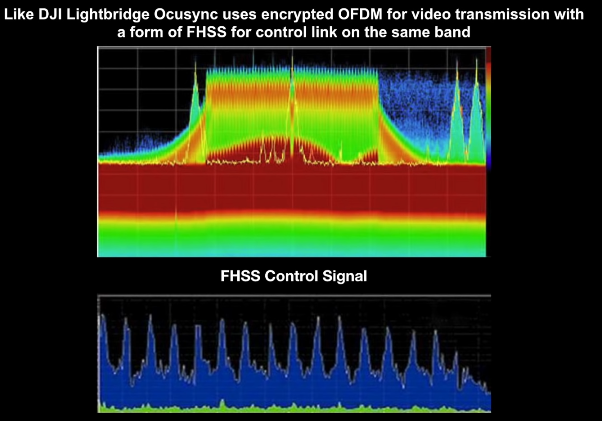
\includegraphics[width=14cm]{Obrazy/ocusync_spectrum_1.png}
\caption{Widmo OFDM i FHSS\cite{ocusync-yt}}
\end{figure}

\begin{figure}[!htbp]
\centering
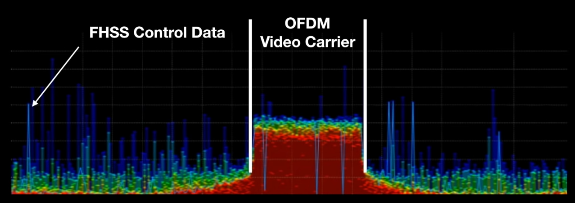
\includegraphics[width=14cm]{Obrazy/ocusync_spectrum_2.png}
\caption{Widmo OcuSync z zaznaczoną modulacja FHSS i OFDM\cite{ocusync-yt}}
\end{figure}


\begin{figure}[!htbp]
\centering
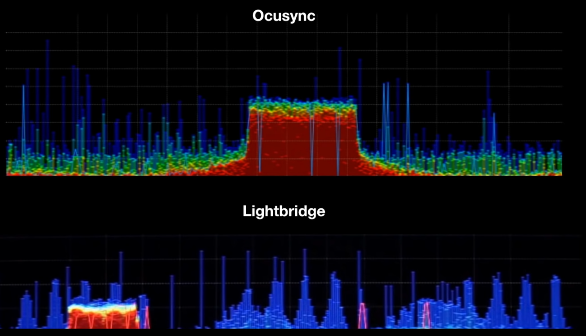
\includegraphics[width=14cm]{Obrazy/ocusync_vs_lightbridge.png}
\caption{Porównanie widma OcuSync i Lightbridge \cite{ocusync-yt}}
\end{figure}

\newpage

\subsection{Przewaga OcuSync nad Lightbridge}
\hspace{1cm}OcuSync stało się główną technologią rozwijaną przez DJI, ponieważ wykorzystuje ono istniejące układy scalone przeznaczone do komunikacji WiFi. Producent wytwarza na nie swoje własne oprogramowanie, które możne następnie aktualizować. Lightbridge był ich własnym układem scalonym, którego oprogramowania nie można było aktualizować, w dodatku komunikacji opierała się wyłącznie na paśmie 2,4GHz. Nowe procesory w układach WiFi dzięki coraz większej częstotliwości pracy zapewniły osiąganie tych samych efektów co Lightbridge, bez dodatkowego kosztu wynikającego z produkcji własnego układu scalonego. 

\section{Sterowanie dronami za pomocą API dostarczaonego od producenta}
\hspace{1cm}Przeszukując internet w poszukiwaniu bezzałogowych statków powietrznych umożliwiających ich sterowanie za pomocą API od producenta można napotkać głównie rozwiązania od DJI. Wszystkie pozostałe rozwiązania nie działają na gotowych dronach, a na oprogramowaniu przeznaczonym do wgrania na wybranych jednostkach do sterowania  modelami RC. 

\hspace{1cm}Najpopularniszym tego rozwiązaniem jest ArduPilot, czyli pakiet oprogramowania nawigacyjnego działającego w pojezdie wraz z oprogramowaniem sterującym stacją naziemną. 

\subsection{DJI SDK}
\hspace{1cm}DJI dostarcza do swoich produktów następujące interfejsy API:
\begin{itemize}
  \item \textbf{App Dev.} - interfejsy API przeznaczone do sterowania dronem z poziomu stacji bazowej, kontroler stanowi interfejs pośredniczący między aplikacją wykorzystującą SDK a dronem powietrznym:\begin{enumerate}
    \item \textbf{Mobile SDK} - SDK przeznaczona na platformę iOS i Android. Aplikacja na smartfon za pomocą kabla USB podłączonego do kontrolera statku powietrznego realizuje zaprogramowaną logikę działania.
    \item \textbf{UX SDK} - Mobile SDK rozszerzony o elementy interfejsu użytkownika, co przyspiesza znacznie proces tworzenia oprogramowania.
    \item \textbf{Windows SDK} - SDK umożliwiające wydawanie aplikacji na systemach operacyjnych Windows. 
  \end{enumerate}
  \item \textbf{Payload Dev.} - interfejsy API przeznaczone do nadawania logiki działania drona na poziomie samego drona, dzięki temu po utracie zasięgu może ona dalej funkcjonować zgodnie z zaprogramowaną logiką. Opcja dostępna dla najdroższych wersji dronów DJI, które można dostosowywać do swoich wymagań za pomocą odpowiednich rozszerzeń, np. kamery termowizyjnej\begin{enumerate}
    \item \textbf{Payload SDK} - zestaw narzędzi programistycznych umożliwiających tworzenie oprogramowania do rozszerzeń, które mogą być montowane na dronach DJI. 
    \item \textbf{Onboard SDK} - otwarto źródłowa umożliwiająca komunikacje bezpośrednia z wybranymi dronami i kontrolerami za pomocą interfejsu szeregowego.  
  \end{enumerate}
\end{itemize}

\chapter{Projekt mobilnego systemu zarządzania i sterowania BSP}
\section{Wymagania funkcjonalne}
\hspace{1cm}text
\section{Wymagania pozafunkcjonalne}
\hspace{1cm}text
\section{Stos technologiczny}
\hspace{1cm}text
\subsection{Java}
\hspace{1cm}text
\subsection{Kotlin}
\hspace{1cm}text
\subsection{DJI Mobile SDK}
\hspace{1cm}text
\subsection{Lombook}
\hspace{1cm}text
\subsection{Springboot}
\hspace{1cm}text
\subsection{Android}
\hspace{1cm}text
\section{Uzasadnienie warstwy pośredniczącej}
\hspace{1cm}text
\section{Wysokopoziomowy diagram systemu}
\hspace{1cm}text
\section{Diagram komponentów}
\hspace{1cm}text
\section{Diagram klas i sekwencji}
\hspace{1cm}text
\subsection{Gradle}
\hspace{1cm}text
\section{Wykorzystane urządzenia}
\hspace{1cm}text

\chapter{Implementacja systemu}
\hspace{1cm}text

\chapter{Testy systemu oraz prezentacja użycia na wybranym case study}
\hspace{1cm}text
\section{Scenariusz testowy autonomicznego lotu pomiędzy dwoma punktami}
\hspace{1cm}text
\section{Scenariusz testowy autonomicznego lotu patrolowego}

% \begin{lstlisting}[caption=Metoda save\_sample()]
% @staticmethod
% def __save_sample(item, tmp_sample: pd.DataFrame, data_type):
%     file_name = InvestingDownloader.__get_file_name(item, data_type)
%     tmp_sample.sort_index(inplace=True)
%     tmp_sample.to_csv('tmp_model_settings.csv')
%     db = pymongo.MongoClient("mongodb://127.0.0.1:27017/")["database"]
%     fs = gridfs.GridFS(db)
%     with fs.new_file(filename=file_name) as fp:
%         fp.write(open('tmp_model_settings.csv', 'rb'))
            
% \end{lstlisting}


\begin{thebibliography}{999}

\bibitem{NB-IoT_vs_Lora}
\bibTitle{NB-IoT vs Lora}
\url{https://ubidots.com/blog/lorawan-vs-nb-iot/#lorawan-vs-nb-iot-a-quick-overview}

\bibitem{m2m-web}
\bibTitle{machine-to-machine (M2M)}
\url{https://www.techtarget.com/iotagenda/definition/machine-to-machine-M2M}

\bibitem{LPWA-wiki}
\bibTitle{LPWA wikipedia}
\url{https://pl.wikipedia.org/wiki/LPWAN}

\bibitem{LoRa-article}
\bibTitle{LoRa Technology - An Overview, IEEE, 2018}
\url{https://ieeexplore.ieee.org/document/8474715}


\bibitem{nbiot-article}
\bibTitle{On the Performance of Narrow-band Internet of
Things (NB-IoT) for Delay-tolerant Services, IEEE, 2019}
\url{https://ieeexplore.ieee.org/document/8768871}

% \bibitem{chollet} F. Chollet,
% \bibTitle{Deep Learning. Praca z językiem Python i biblioteką Keras}, Helion,  2019;

\bibitem{dji-wiki}
\bibTitle{Wikipedia: SZ DJI Technology Co., Ltd.},
\url{https://pl.wikipedia.org/wiki/DJI}, 2022;

\bibitem{dji-mavic-mini-se-spec}
\bibTitle{DJI Mavic Mini SE},
\url{https://www.dji.com/pl/mini-se?site=brandsite&from=nav}, 2022;

\bibitem{dji-store}
\bibTitle{DJI store},
\url{https://store.dji.com}, 2022;

\bibitem{lightbridge-dji}
\bibTitle{DJI Lightbridge},
\url{https://www.dji.com/pl/dji-lightbridge/info}, 2022;

\bibitem{lightbridge2-dji}
\bibTitle{DJI Lightbridge2},
\url{https://www.dji.com/pl/lightbridge-2/info#specs}, 2022;

\bibitem{OFDM-wiki}
\bibTitle{Wikipedia: OFDM},
\url{https://pl.wikipedia.org/wiki/OFDM}, 2022;

\bibitem{FHSS-wiki}
\bibTitle{Wikipedia: FHSS},
\url{https://pl.wikipedia.org/wiki/FHSS}, 2022;

\bibitem{ocusync-yt}
\bibTitle{DJI Mavic 2 - Ocusync 2.0 What is it \& What's Compatible ? + How is it different from Lightbridge},
\url{https://www.youtube.com/watch?v=gfqcSv9sR0A}, 2022;

\bibitem{dji-gogle}
\bibTitle{DJI Gogle},
\url{https://u.cyfrowe.pl/600x0/2/7/2_732250420.png}, 2022;

% \bibitem{sghblockchain}
% \bibTitle{Blockchain. Kolejny etap cyfrowej rewolucji?},
% \url{https://ssl-administracja.sgh.waw.pl/pl/br//gazeta/archiwum/Documents/342_wiosna_2018_blockhain.pdf/}, 2018;

% \bibitem{dash}
% \bibTitle{Introduction to Dash},
% \url{https://dash.plotly.com/introduction}, 2021;

% \bibitem{oreilly} D. Osinga,
% \bibTitle{Deep Learning. Receptury}, Helion,  2019;

% \bibitem{valentino} Valentino Zocca, Gianmario Spacagna, Daniel Slater, Peter Roelants,
% \bibTitle{Deep Learning. Uczenie głębokie z językiem Python. Sztuczna inteligencja i sieci neuronowe}, Helion,  2018;

% \bibitem{oreilly} D. Osinga,
% \bibTitle{Deep Learning. Receptury}, Helion,  2019;

% \bibitem{zrozumiec_bitcoina} Silas Barta, Robert P. Murphy,
% \bibTitle{Zrozumieć Bitcoina. Techniczn i ekonomiczny przewodnik po kryptowalutach}, Fijorr,  2018;

% \bibitem{zrozumiec_bitcoina} Anna Iwona Piotrowska,
% \bibTitle{Bitcoin. Płatnicze i inwestycyjne zastosowania kryptowaluty}, CeDeWu,  2018;


\end{thebibliography}

\listoffigures

\listoftables

\end{document}
